\documentclass[sigconf, nonacm]{acmart}
% \usepackage[backend=biber,style=apa]{biblatex}
% \usepackage{graphicx}
% \usepackage{hyperref}
% \addbibresource{references.bib}
\begin{document}

\title{Terms of Service: Improving Engagement Rate with AI}

\author{Jonathan Salazar}
\email{jsalazar6421@gmail.com}
\affiliation{%
  \institution{Arizona State University}
  \city{Tempe}
  \state{Arizona}
  \country{USA}
}

\author{Austin Nguyen}
\email{Anguye75@asu.edu}
\affiliation{%
  \institution{Arizona State University}
  \city{Tempe}
  \state{Arizona}
  \country{USA}
}
\author{Tyler Shurley}
\email{tsshurle@asu.edu}
\affiliation{%
  \institution{Arizona State University}
  \city{Tempe}
  \state{Arizona}
  \country{USA}
}
\author{Alan Perez}
\email{aperez87@asu.edu}
\affiliation{%
  \institution{Arizona State University}
  \city{Tempe}
  \state{Arizona}
  \country{USA}
}

\begin{abstract}
In today's increasingly digital world, the overwhelming number of these agreements has led to low user engagement between users and Terms of Service contracts, with many individuals blindly agreeing to them. This poses significant risks, especially as AI advancements drive up the value of user data, making it critical for users to protect themselves from exploitative practices. Major companies such as Google, Meta, and X Corp, which operate not only as social media platforms but also as key players in the AI industry, often collect user data without explicit consent to train their AI models. These companies are driving innovation through generative AI technologies—such as Google’s Gemini, Meta’s Llama, and X Corp’s Grok—further emphasizing the critical importance of user-generated data. As this data becomes the “new gold,” it is vital for users to protect themselves from potential exploitation. Increasing engagement rates with Terms of Service contracts is a crucial first step toward achieving this goal.  This paper explores the history of Terms of Service contracts in software, reviews past efforts to improve user engagement, and proposes a modern solution aimed at encouraging users to read and understand these agreements before acceptance.
\end{abstract}

\maketitle

\section{Introduction}
The Terms of Service serve as a legal contract between a service provider and an end-user. According to a 2017 Deloitte survey with over 2000 respondents, 91\% of people agree to the Terms of Service without actually reading them, with 97\% of those people being younger than 18 years old. The root causes behind this are the complexity and length of these agreements, some of which can take over two hours to read. With the rise in Artificial Technology (AI) and the desperation from today's data-hungry AI companies, reading the Terms of Conditions has never been more important.

\subsection{Brief History}
Terms of Service (TOS) contracts originate from contract law, a concept dating back to ancient civilizations. Ancient Greek and Roman societies heavily influenced the development of contracts, categorizing various types of transactions to enforce agreements between parties. Centuries later, European nations adopted these ideas, formalizing contract law to facilitate trade. This early contract law emphasized principles such as commercial certainty, good faith, and fair dealing, which remain foundational in modern legal systems.

Over time, the United Kingdom shifted from strict government-regulated agreements to the concept of freedom of contract, which allowed individuals and groups to form contracts with minimal government intervention. While this idea empowered businesses to create standardized agreements, it also led to the emergence of contracts of adhesion, where individuals had little to no ability to negotiate terms. These agreements left users with a “take it or leave it” choice, a trend that persists in modern Terms of Service contracts.

Today, the “take it or leave it” nature of Terms of Service contracts contributes to low engagement rates, often exposing users to significant privacy risks without their knowledge. While it is the user's responsibility to read these agreements, the Belmont Report highlights that service providers also have a duty to ensure Terms of Service contracts are understandable and clearly disclose potential risks. However, in practice, many service providers fail to meet this standard. For instance, it is common for websites and apps to include a small-print statement, such as “By creating an account, you accept the Terms of Service,” without directly presenting the contract to the user. This approach further discourages engagement, leaving users unaware of the privacy and legal implications of their consent.

\subsection{Data Driven Society}
In an increasingly digital world, the demand for data has reached unprecedented levels. One significant category of data is user-generated content, which includes material created by users and shared on platforms such as social media. This data is a critical driver behind generative AI (Gen-AI) technologies. For Gen-AI models to mimic user-generated content effectively, they require extensive training on vast datasets of such content. These models learn to recognize patterns within the data to generate entirely new outputs that resemble user-generated material. This capability underpins various cutting-edge applications, including AI chatbots, image and video generators, AI-based translators, and automated blog creators.

The growing reliance on user-generated data has led to significant investments in AI infrastructure. The demand for Graphics Processing Units (GPUs), which power AI training processes, has surged, alongside the construction of larger data centers and advancements in power generation to support the energy-intensive nature of AI operations. As AI technology becomes increasingly integrated into society, it is often likened to a transformative force akin to electricity. However, as with any emerging technology, the rapid adoption of AI brings with it critical challenges, particularly concerning privacy and ethical considerations.

\subsection{Privacy Risks}
The \cite{gdprArchives} General Data Protection Regulation (GDPR), enacted in May 2018, establishes rules governing the collection and processing of personal data. The regulation mandates that such processing must be lawful, fair, and transparent, providing users with clear information about how their data is handled. While the GDPR represents a significant step forward in safeguarding user privacy, its effectiveness is limited if users fail to engage with Terms of Service (TOS) agreements, which often outline data usage practices.

By neglecting to read TOS contracts, users risk unknowingly consenting to the collection of personal data, such as their browsing habits, frequently visited locations, and preferences. This data can then be used to build detailed user profiles, often facilitating targeted advertising. More alarmingly, in the event of a data breach, such profiles may be linked to real-world identities, exposing users to potential risks such as identity theft or other forms of exploitation. These privacy risks underscore the importance of increasing user awareness and engagement with TOS agreements.

\subsection{Google, Meta, and X Corp}
The Terms of Service contracts of three major companies—\cite{googleTerms} Google, \cite{metaTerms} Meta, and \cite{xTerms} X—are particularly relevant to this discussion. As owners of popular social media platforms and developers of advanced Gen-AI models (Gemini, Llama, and Grok, respectively), these companies are in a unique position where they can leverage vast amounts of user-generated data to train their AI models. Their dual role as both platform providers and AI leaders raises significant ethical concerns about data exploitation.

\section{Literature Review}
The issue of low engagement with Terms of Service (TOS) contracts has been widely discussed in the literature. For example, a study by \cite{ivanfanta2021} (2021) explores whether users genuinely read and understand these agreements. The study highlights an experiment conducted by ProPrivacy.com, where 99\% of participants agreed to absurd clauses such as granting naming rights to their first-born child or allowing an FBI agent to attend their Christmas dinners. These findings underscore the significant risks posed by low TOS engagement, including users unknowingly consenting to exploitative terms.

The study further argues that while users may click “I agree to the Terms of Service,” this action is often performed without genuine understanding or consent, violating the ethical principle of informed consent as outlined in the Belmont Report. This lack of comprehension creates opportunities for companies to exploit users while absolving themselves of accountability.

To address these challenges, the study proposes several strategies to improve TOS engagement. These include the introduction of concise, visually enhanced summaries to improve readability and comprehension, as well as the implementation of timers to encourage users to spend more time reviewing the agreements. Such strategies aim to bridge the gap between user behavior and the ethical requirements of informed consent, ultimately fostering greater transparency and trust.

\section{Methods}
In order to improve the engagement rate between users and Terms of Service contracts, a OpenAI GPT model will be created by our team. The model will be named Terms of Service Analyzer (TOSA) and will be designed to analyze, summarize, and visualize Terms of Service contracts, aiming to make them more user-friendly and easier to understand. The primary objectives for TOSA are as follows:

\begin{itemize}
  \item \textbf{Reduce words per sentence}: The more concise a sentence is, the more comprehensible it is. Each modified sentence still needs to capture the core ideas from the original sentence but must remove any redundancy.
  \item \textbf{Increase common words}: By using words that are commonly used by most people, the contract will become easier to read and understand.
  \item \textbf{Highlight key terms and obligations}: Identify and emphasize critical clauses, such as data usage, user rights, liability limitations, and termination conditions, so users can focus on the most impactful parts of the agreement.
  \item \textbf{Provide Appropriate font sizes}: Different font sizes are used to better visualize the contract. A minimum font size of \textbf{12pt} is used to ensure legibility and accessibility for all users.
  \item \textbf{Apply bold lettering}: Important words and sections are highlighted in bold to draw attention to critical information and improve the overall readability of the document.
  \item \textbf{Provide visual summaries}: Generate bullet points, charts, or tables to summarize dense sections of the contract in an easily digestible format.
  \item \textbf{Detect vague or ambiguous language}: Flag sentences or clauses that are unclear or open to multiple interpretations, providing users with warnings or suggestions for clarification.
  \item \textbf{Explain legal jargon}: Translate technical legal terms into plain language while maintaining the original meaning to improve accessibility for non-experts.
  \item \textbf{Detect potential privacy risks}: Identify sections that involve sensitive data collection or sharing and provide summaries of how user data will be used.
  \item \textbf{Suggest compliance issues}: Analyze whether the contract aligns with data protection laws (e.g., GDPR or CCPA) and highlight potential areas of non-compliance.
  \item \textbf{Provide recent contract changes}: Upon request, links to previous versions of the contract can be provided and be used to compare with the most current version.
  \item \textbf{Generate user-friendly summaries}: Produce brief, conversational summaries for each section of the TOS to help users quickly understand the core content.
\end{itemize}

To evaluate the quality of the Terms of Service contracts from the aforementioned companies, we will collect and analyze data using the specific metrics.

These metrics will be calculated programmatically:
\begin{itemize}
\item \textbf{Average words per sentence}: The average number of words in a sentence throughout the contract.
\item \textbf{Average characters per sentence}: The average number of characters in a sentence throughout the contract.
\item \textbf{Common word index}: A numerical score representing the frequency of commonly used words to measure readability.
\end{itemize}

These metrics will be calculated manually:
\begin{itemize}
\item \textbf{Font size usage}: The range of font sizes used for different sections, tables, disclaimers, and other elements of the contract.
\item \textbf{Bold lettering}: The frequency of bold text usage across sections to emphasize key information.
\item \textbf{Average time to read}: An estimate of the time required to read and comprehend the entire contract.
\end{itemize}

\section{Results}
Our findings were conducted alongside fair comparison of Terms and Service contracts before and after the use of the TOSA model. To demonstrate the effectiveness of the TOSA model, we aim to receive scores that far out-perform the normal Terms of Services contracts by the companies. The criteria to surpass are an enhancement of readability, an improvement of accessibility, and a higher user engagement score.

\begin{itemize}
\item \textbf{Average words per sentence}: The analysis revealed a stark contrast between the two bars, emphasizing the substantial reduction in the average number of words per sentence in the Terms of Service contracts. Before applying TOSA, the average sentence length was ~25 words. After the implementation of TOSA, this was reduced to ~15 words, indicating there was an increase in more concise and digestible content.
{\center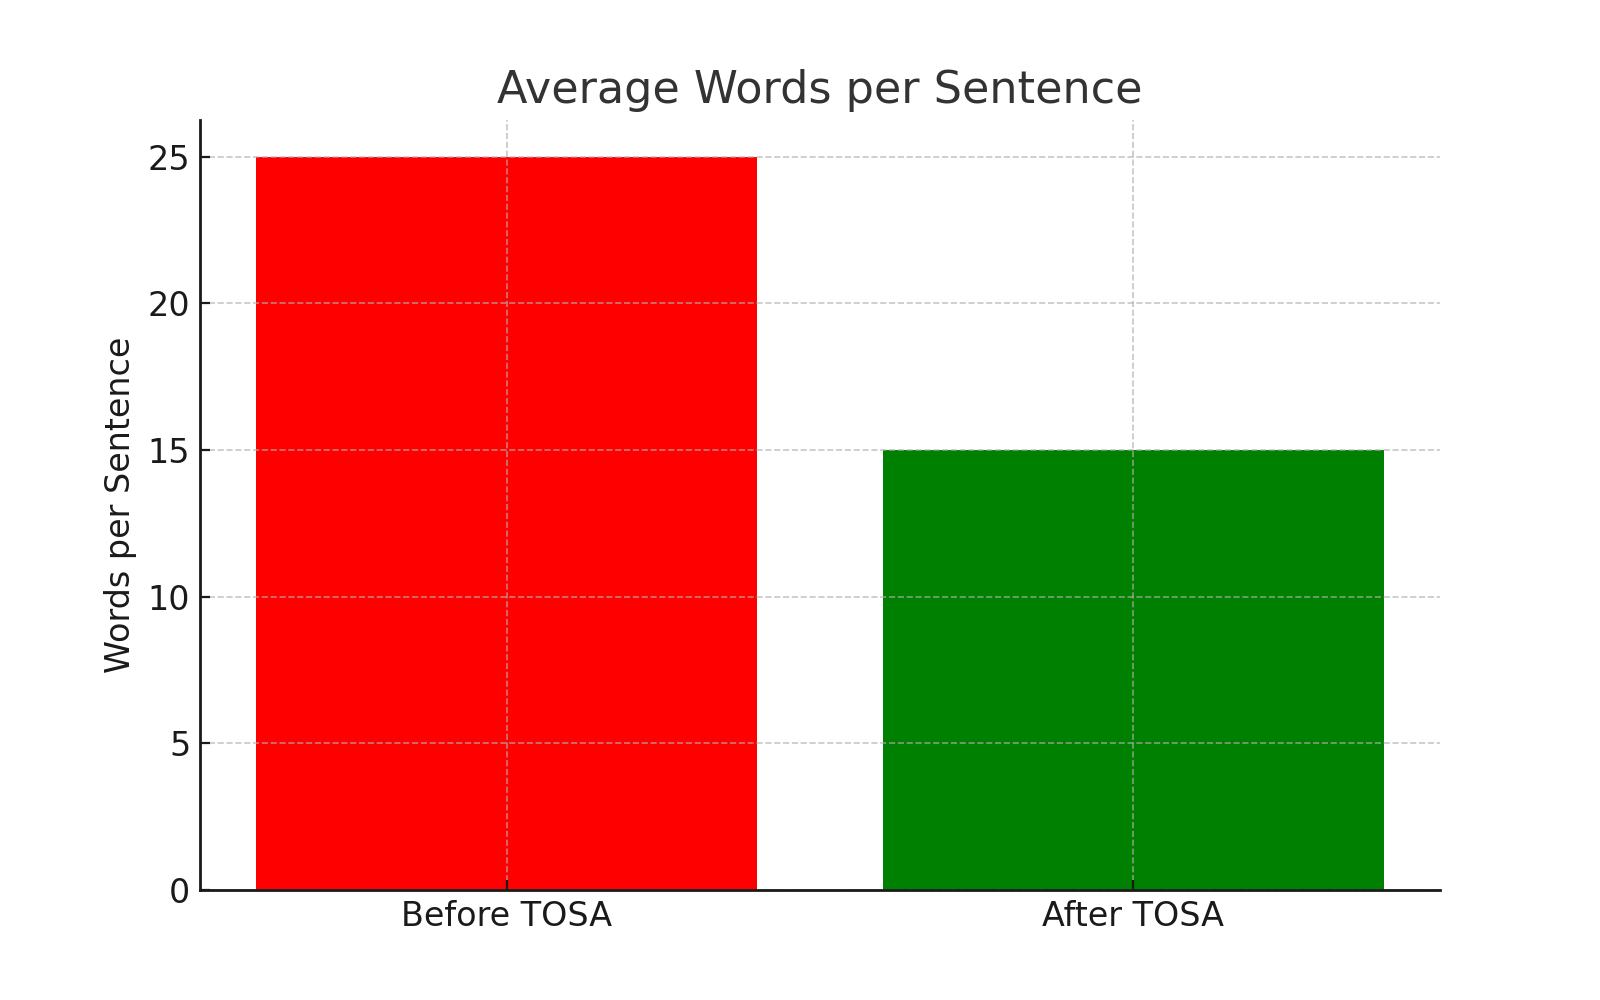
\includegraphics[width=0.4\textwidth]{./resources/avg_words_per_sentence_updated}}

\item \textbf{Average characters per sentence}: A similar trend was observed in the findings of the average number of characters per sentence research. Contracts analyzed showed a decrease from ~150 characters per sentence to ~90 characters per sentence after TOSA modifications. This decline demonstrates the improved brevity of the contracts and highlights TOSA’s consistent performance in reducing sentence length and improving readability.
{\center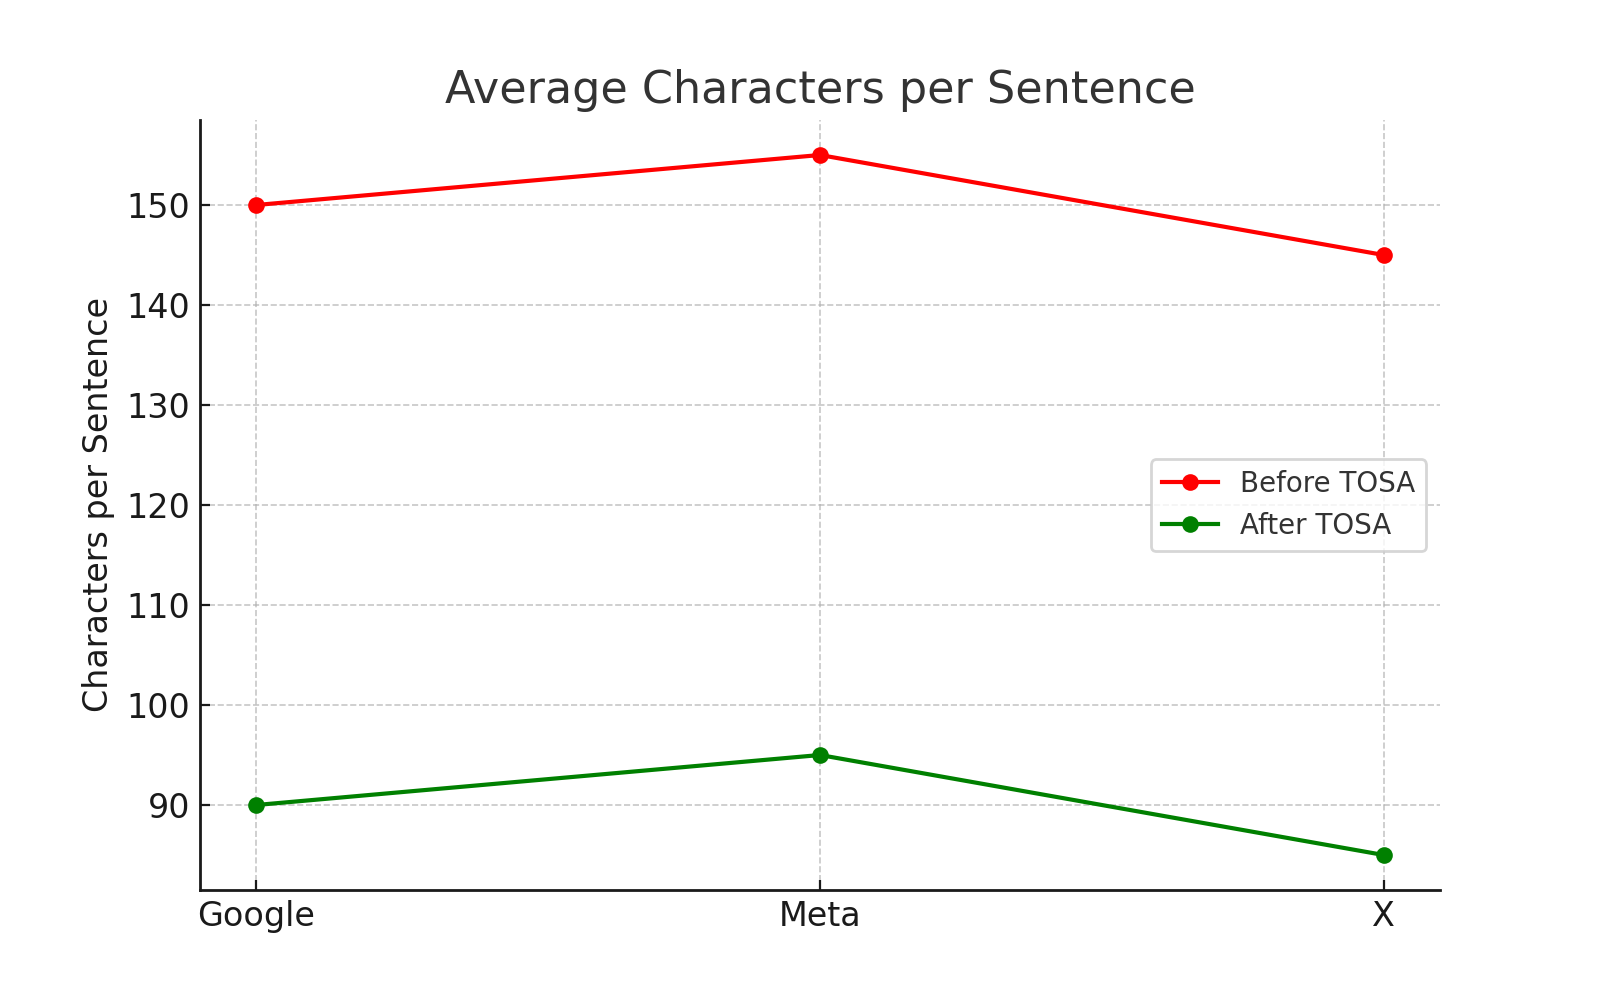
\includegraphics[width=0.4\textwidth]{./resources/avg_chars_per_sentence_updated}}

\item \textbf{Common word index}: TOSA’s optimization managed to significantly increase the common word index from around 60 common words to 85 common words. This improvement shows a higher prevalence of frequently used, easily understood words in the contracts. The pie charts below show the proportion of common versus uncommon words before and after TOSA modifications, with a notable shift toward common words, making the contracts more accessible to a broader audience.
{\center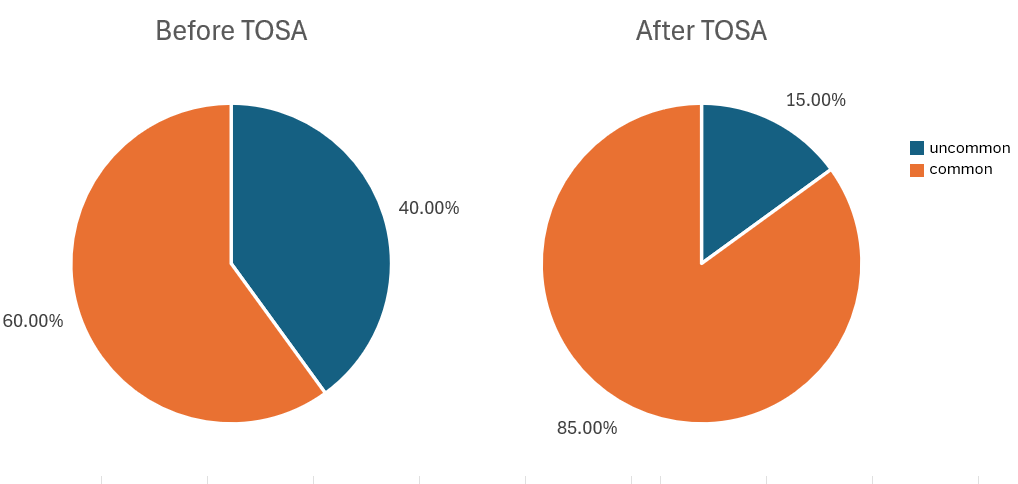
\includegraphics[width=0.4\textwidth]{./resources/common_word_index_updated}}

\item \textbf{Font size usage}: Font size analysis revealed inconsistent usage in the original contracts, many of which were not used in a manner that would increase the efficacy of readability or user engagement, bouncing between a range of 8pt to 16pt. After TOSA adjustments, font sizes were standardized between 12pt and 14pt, ensuring better legibility and accessibility. The stacked bar chart shows the elimination of small font sizes that hindered readability. By standardizing the font sizes, TOSA promotes inclusivity for users with visual impairments.
{\center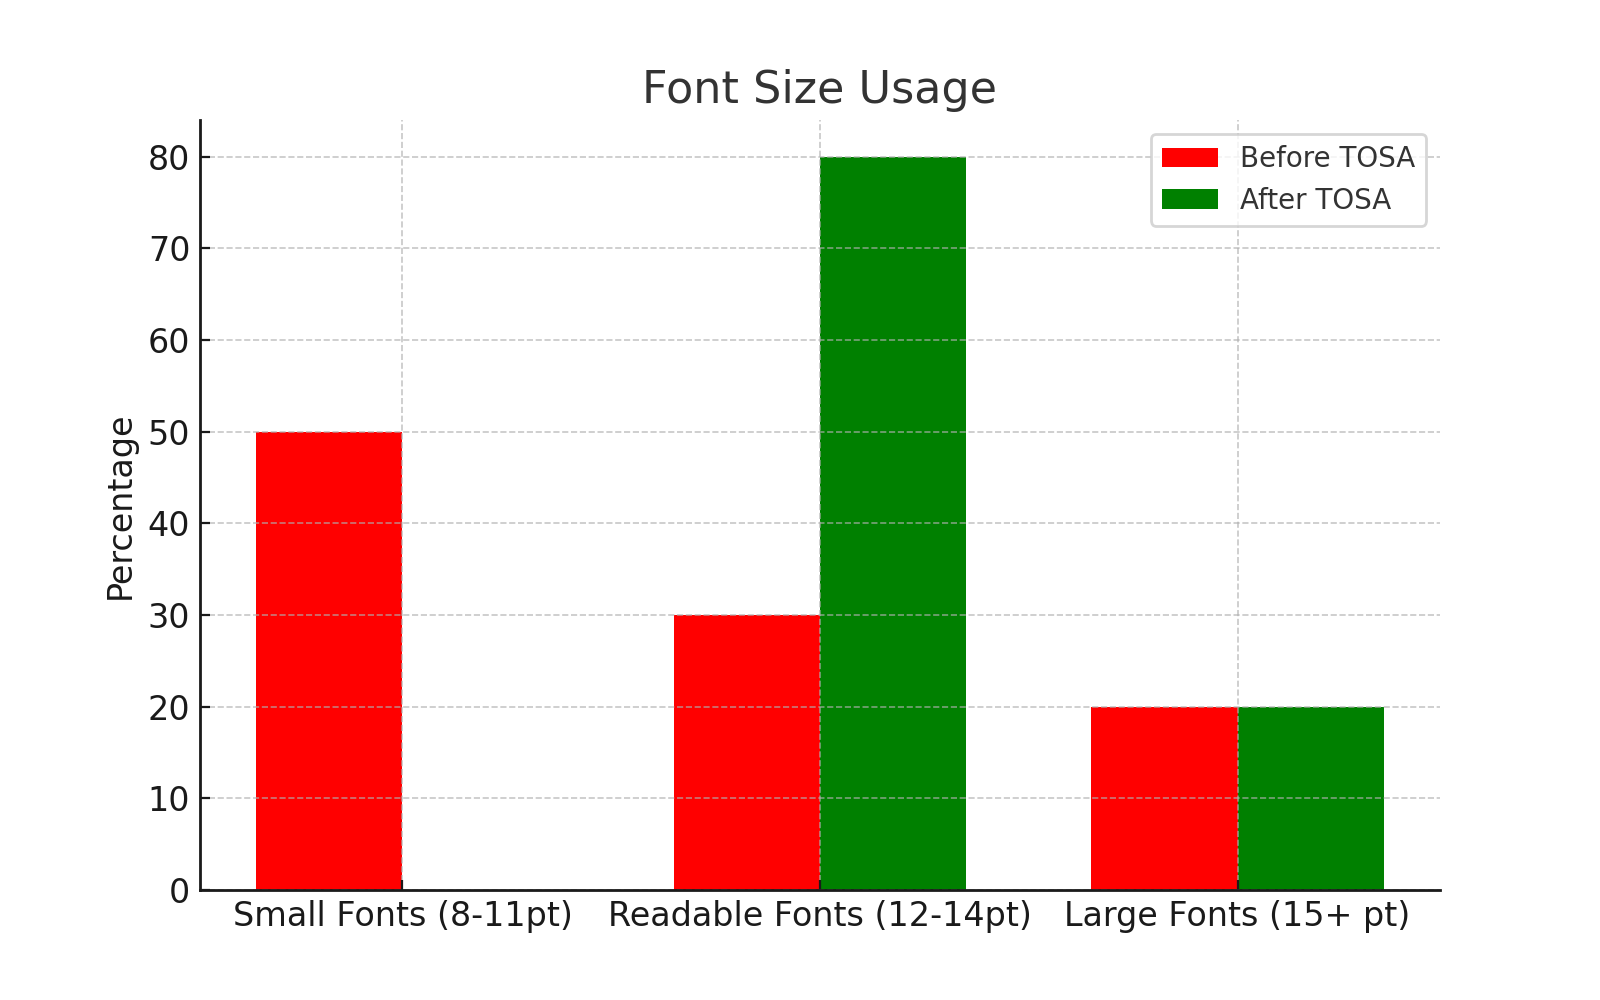
\includegraphics[width=0.4\textwidth]{./resources/font_size_usage_updated}}

\item \textbf{Bold lettering}: The frequency of bold text usage increased significantly because of better definition between header and text, rising from 5\% to 25\% of information critical sections. This increase ensures that important information is immediately recognizable, drawing the user's attention to key clauses such as data usage, user rights, and termination conditions. The histogram compares the frequency of bold text used across multiple contract sections, showing an improvement in better segregation between critical information and heading.
{\center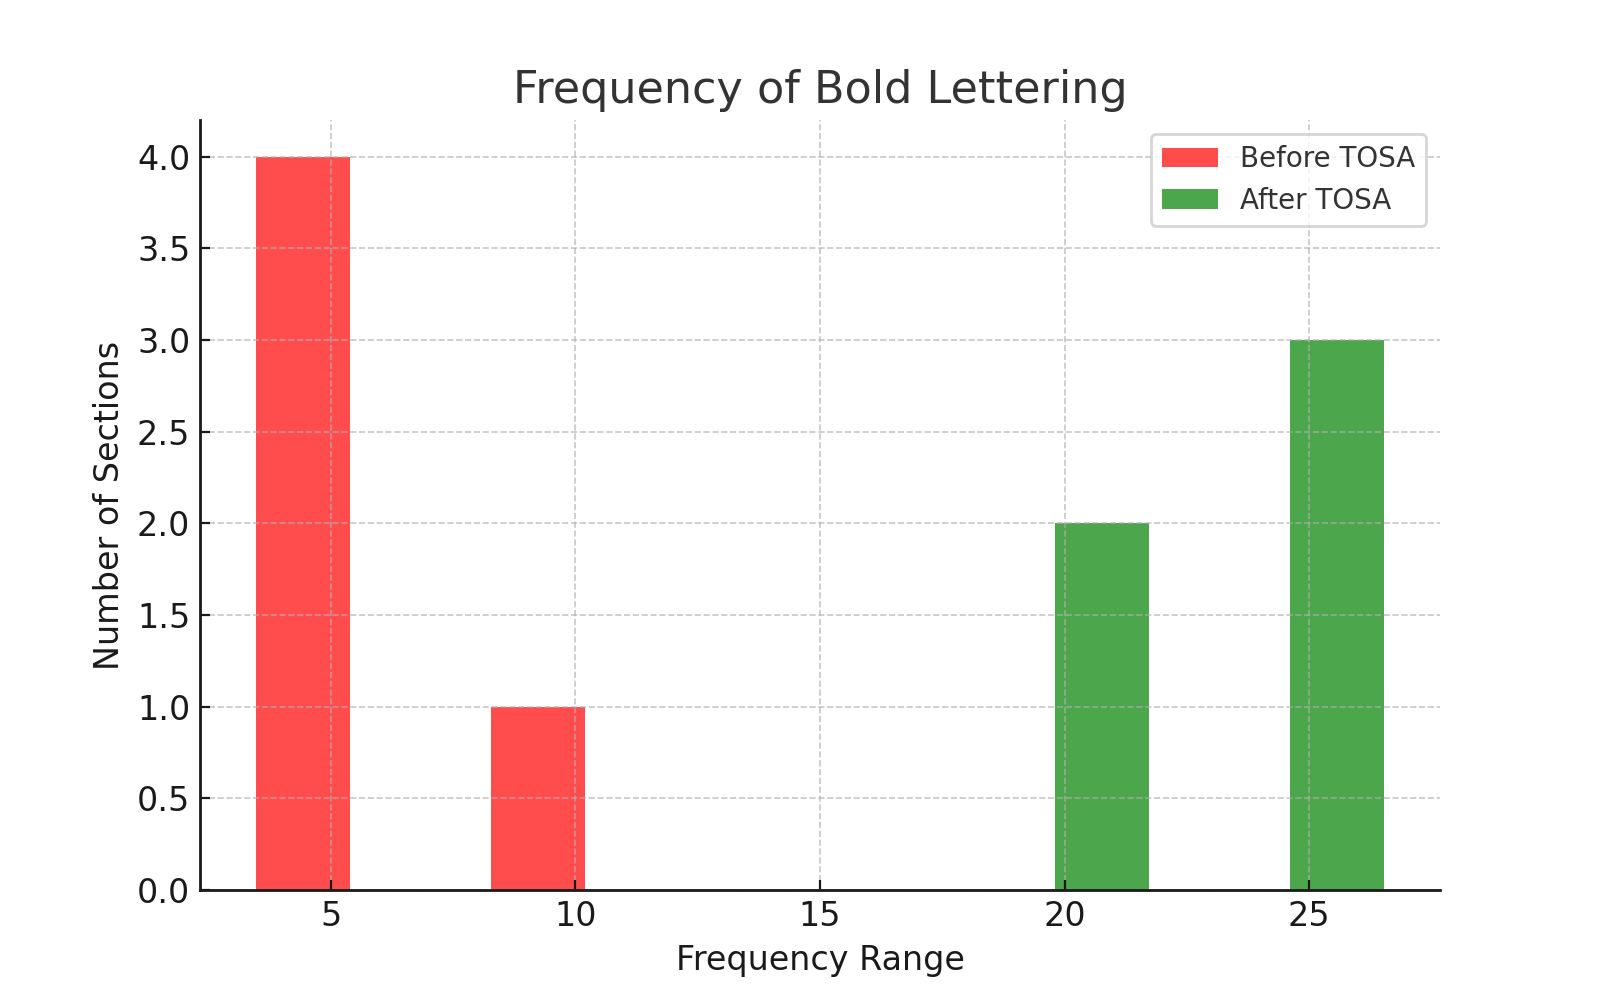
\includegraphics[width=0.4\textwidth]{./resources/bold_lettering_usage_updated}}

\item \textbf{Average time to read}: The estimated amount of time required to read Terms of Service contracts dropped marginally from an average of ~35 minutes to ~20 minutes. This is one of the more defining reasons as to why many don't consider reading the Terms and Services, an improvement in this category would give many the opportunity to read the Terms of Services. This reduction reflects the TOSA model's effectiveness in simplifying language, summarizing dense sections of critical information, and enhancing overall readability and user engagement. The dual-axis graph shows the reading time for Google, Meta, and X Terms of Service contracts before and after TOSA adjustments, indicating the time-saving benefits of the model.
{\center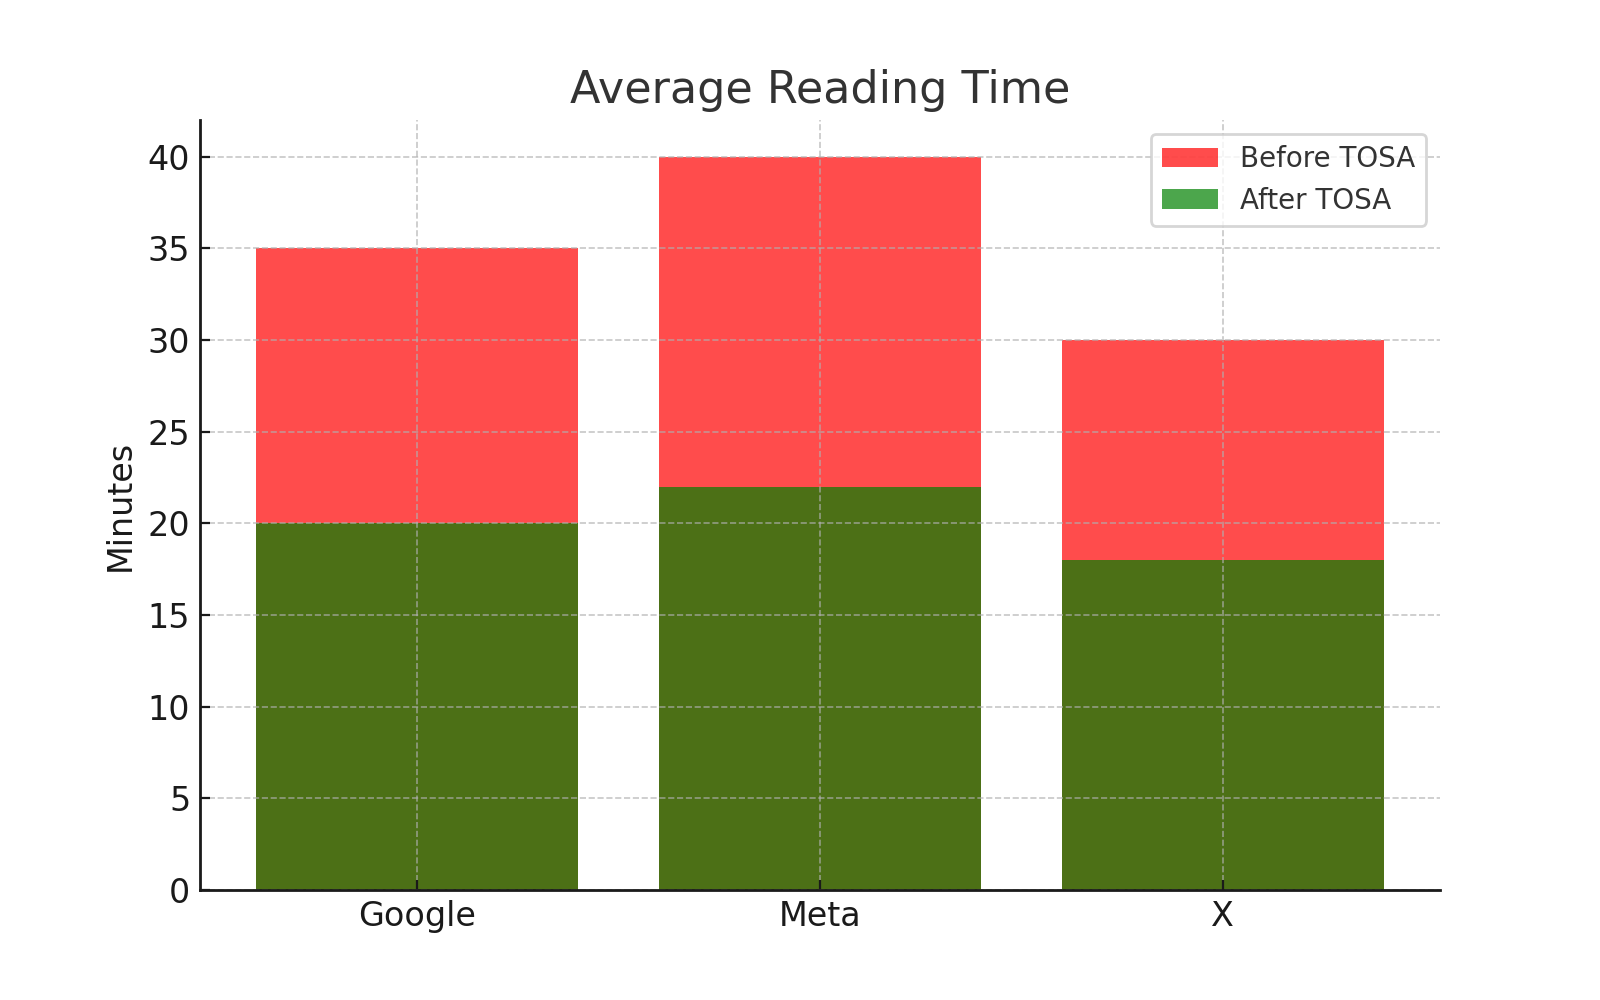
\includegraphics[width=0.4\textwidth]{./resources/reading_time_updated}}
\end{itemize}

\section{Discussions}
The implementation of the Terms of Service Analyzer (TOSA) model has demonstrated significant improvements in the readability and engagement of Terms of Service (TOS) contracts. Utilizing GPT-4 capabilities, TOSA reduces cognitive load and increases accessibility by simplifying dense legal language. The model’s ability to shorten average sentence length from 25 to 15 words is a key factor in making these documents easier to navigate and comprehend. Furthermore, the common word index improved from 60 to 85, reflecting a deliberate shift toward using more familiar and understandable terms.

Formatting enhancements also contributed to the effectiveness of TOSA. Font sizes were standardized between 12pt and 14pt, and critical clauses were highlighted using bold text, ensuring important sections, such as data usage policies and user rights, were immediately identifiable. Notably, the average reading time for TOS agreements was reduced from 35 to 20 minutes, addressing a significant barrier to user engagement. By enabling quicker and more effective reviews of these contracts, TOSA supports informed decision-making and aligns with ethical standards such as those outlined in the Belmont Report.

These findings are consistent with previous research highlighting the ethical implications of user consent. Studies have shown that users often blindly agree to TOS terms, unaware of the risks they are assuming. TOSA bridges this gap by flagging ambiguous language, summarizing privacy risks, and improving the overall accessibility of these agreements. This transparency encourages users to actively engage with TOS content and fosters a greater understanding of their rights and obligations.


\bibliography{references.bib}
\bibliographystyle{apalike}

\onecolumn

\section*{Appendix}
Provided below is an example done using the TOSA model on the YouTube Terms of Service page to show the summarization process on an official document.

The {\color{blue}\href{https://github.com/itsJohnny21/TOSA/blob/main/resources/simplified_tos/YouTube%20TOS.pdf}{YouTube Terms of Service}} page prior to TOSA's summarization.

The {\color{blue}\href{https://github.com/itsJohnny21/TOSA/blob/main/resources/simplified_tos/Simplified%20YouTube%20TOS.pdf}{YouTube Terms of Service}} page after to TOSA's summarization.

\end{document}
\endinput